\section{The Interstellar Medium}

I added sections based on the list of important topics Allison gave us 
before the final. 

\subsection{Questions}
\begin{enumerate}
\item \textbf{Draw the cooling function for gas of solar metallicity, and describe the cooling
      mechanisms in each part of the curve. Explain the relevance of this function to multi-
      phase ISM models.}
      
      The figure below shows the cooling function $\Lambda$ as a function of $T$ (note that in class, Nick showed us a cooling curve of $T$ vs. $n$). At $T < 10^3$ K, the cooling is from molecular line emission. The plateau from $\sim10^3$ to $\sim10^4$ K is due to collisionally excited lines of neutral and low-ionization metals. There is a peak around $\sim10^4-10^5$ K, which is due to recombination of hydrogen (i.e. hydrogen recombines and then downward transitions emit low-energy photons such as H$\alpha$ that find the HII region optically thin). There is a quadruple peak at $T \approx 10^5,~2\times 10^5,~5\times 10^5,~10^6$ K from far-UV and X-ray emission lines from highly ionized species of C,O,Ne,Fe, respectively. At $T > 10^7$ K, most of the cooling is from Bremsstrahlung.
      
            \begin{figure}[!h]
      \begin{center}
      \includegraphics[width=\textwidth]{ism_Q1_cool.jpg}
      \end{center}
	\end{figure}
	
	Below is a more detailed version from Nick's notes, and it goes to higher temperature.
	
	  \begin{figure}[!h]
      \begin{center}
      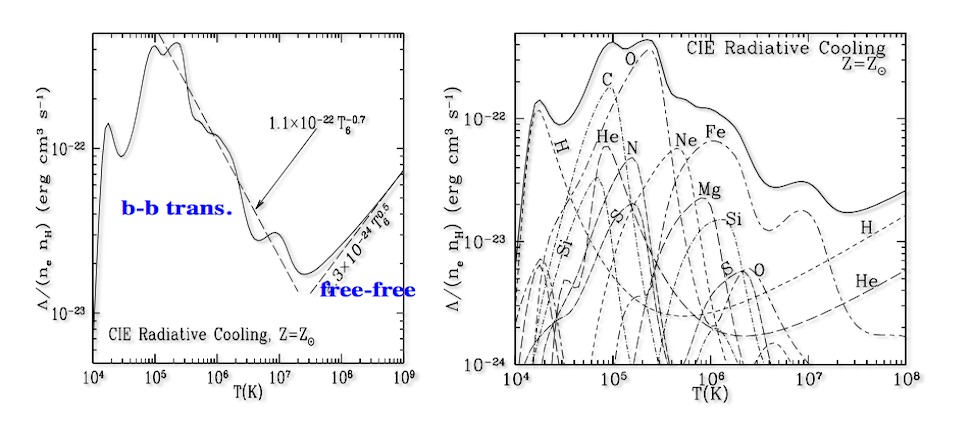
\includegraphics[width=\textwidth]{ism_Q1_cool_b.jpg}
      \end{center}
	\end{figure}
      
\item \textbf{Draw a typical spectrum of an HII region, including both lines and continuum, and
      explain the major processes that give rise to each feature.}
      
      Below is a spectrum of an HII region with the continuum removed. The spectrum is similar to that of a planetary nebula (a ball of mostly-hydrogen gas ionized by the newly formed white dwarf instead of a young star). The hydrogen features are from transitions to the $n=2$ state (no Lyman features are pictured here, but ${\rm Ly}\alpha$ should be there) of 
      
      \begin{figure}[!h]
      \begin{center}
      \includegraphics[width=\textwidth]{ism_Q2_HII_spec.jpg}
      \end{center}
	\end{figure}
\item \textbf{Explain quantitatively what determines the temperature of dust grains and their
      thermal emission spectrum. Give examples of astrophysical environments with different
      dust temperatures.}
\end{enumerate}

\subsection{Useful Numbers and Relations}
$2\times10^{21}$ H cm$^{-2}$ for $1$ mag of visual extinction\newline
\newline
$30$ mag of visible extinction towards Galactic Center\newline
\newline
$13.6$ eV=$912$ \AA=shock with v$>50$ km/s\newline
\newline
$\frac{E}{eV}=\frac{T}{10,000 K}$\newline
\newline
H photoionization cross section $\sigma_{\nu}=6\times10^{-18}(\nu/\nu_0)^{-3}
cm^2$\newline
\newline
mean free path = $1/(n\sigma)\sim 1.6\times10^{17}/n_H$ cm\newline
\newline
$v_{sound}=\sqrt{\frac{\gamma kT}{m}}$\newline
\newline
For atomic H and $\gamma=5/3$,\newline
\newline
$\frac{v_{sound}}{km/s}=\sqrt{\frac{T}{100 K}}$

\subsection{Basic Things about ISM Phases}

The ISM phases are characterized by the state of hydrogen gas.

H$_2$ (molecular): $n \sim 200-10^6~{\rm cm}^{-3}$, $T \sim 10-500~{\rm K}$

Exists in molecular clouds and dark clouds, as well as protostellar cores.  
Molecular and dark clouds (lower end of the temperature and density range) are 
detected based extinction of background stars.  Giant molecular clouds 
have temperatures of $50-100$ K and and are heated by newly formed massive 
stars.  These are also seen in extinction, and in line emission in the far-IR 
and radio.  The molecular H itself is very difficult to detect 
spectroscopically, but other molecules in the clouds such as CO can be 
detected.  Giant molecular clouds have masses of 
$10^3-10^6\ M_{\odot}$.  The hottest and densist H$_2$ is found in protostellar 
cores, which are collapsed regions of GMCs.  

HI (atomic): $n \sim 1-100~{\rm cm}^{-3}$, $T \sim 100-3000~{\rm K}$

Atomic H is found in diffuse clouds.  These clouds are semitransparent, with 
visual extinction of $\sim1$ mag.  The are observed using $21$ cm emission 
(warmer clouds) and absorption (cooler clouds).  In the centers of the clouds, 
molecules such as CO and OH can form and be shielded from starlight.  These 
clouds are also visible in the infrared from their blackbody radiation.  
 
HII (ionized): $n \sim 0.1-10^3~{\rm cm}^{-3}$, $T \sim 10^4-10^6~{\rm K}$

Ionized H is found in emission nebulae (planetary nebulae, supernova remnants, 
and HII regions).  Observationally, ionized H can be observed using H 
recombination lines (such as H$\alpha$) and other atomic recombination lines 
such as [OIII].  Bremsstrahlung emission is also seen in these regions.  
Supernova remnants and planetary nebulae have well defined shell-like shapes 
and are associated with individual stars.  HII regions appear fuzzy and 
are associated with sites of multiple star formation and molecular clouds.  
Planetary nebulae can also be distinguished from HII regions from line ratios.  
The star at the center of a planetary nebula is the core of an evolved star, 
and can be $>10^5$ K.  This produces much higher energy photons than those 
in HII regions, so ratios of [OIII] to H$\alpha$ are higher in planetary 
nebulae, and even He recombination lines are weakly visible.  

Ionized H can also be found in galactic coronal gas in the halo.  This gas 
is most likely heated $10^5-10^6$ K gas is most likely heated by shocks from 
multiple supernovae.  It can be detected from X-ray emission and UV absorption.
 
 Transitions between phases:
 
 Ionization of neutral hydrogen requires $13.6~{\rm eV}$, or photons with wavelength $\lambda < 912 \AA$, OR shocks that are faster than $50~{\rm km/s}$. In HII regions around hot (O,B) stars, the hydrogen is photoionized by the UV radiation from the star, and there are very sharp transitions between the HII, HI, and H$_2$ regions around the star.

\subsection{Heating and Cooling}
The example of heating and cooling we did in class was for an HII region.  
According to the slides, the same derivation can be followed for other 
phases of the ISM, just with different transitions.  

In an HII region, gas is heated when a photon with energy $>13.6$ eV ionizes 
a neutral H atom.  This gives the free electron extra kinetic energy, which 
it transfers to the gas.  The rate of heating is just the rate at which 
energy is transferred into the gas by this method.  So the heating rate 
$\Gamma$ is the photo-ionization rate times the extra energy per 
photo-ionization.
\begin{equation}
\Gamma=R_{ph}\times\bar{E}
\end{equation}
Since the HII region is fully ionized, photo-ionizations can only take 
place at the rate of recombinations (this is basically saying ionization 
equilibrium is maintained.  So the rate of photo-ionizations equals the rate 
of recombinations:
\begin{equation}
R_{ph}=n_en_p\alpha_B
\end{equation}
where $\alpha_B$ is the recombination rate coefficient into levels higher than 
n$=1$.  Things get confusing here with these $\alpha$s.  There's a total $\alpha$ 
for all recombinations, an $\alpha_A$ for recombinations to n$=1$, and 
$\alpha_B$.  Kwok says $\alpha_B$ should be used here.  The lecture slides 
say it should be $\alpha_A$, but later in the derivation, it looks like this 
magically turns into $\alpha_B$.  I'm assuming the $\alpha_A$ in the lecture 
slides is a typo, and we should be using $\alpha_B$.  This makes sense 
physically, because we want to know the rate of recombinations that allow 
a photon from the central star to ionize an atom.  If a recombination happens 
directly to n$=1$, then a photon will be emitted with enough energy to 
ionize a new atom.  So the photon from the star that is trying to heat the gas 
will still have nothing new to ionize.  If the recombination happens to a 
higher energy level, and the electron cascades down to n$=1$, several photons 
will be emitted, but none will be able to ionize anything.  So the net result 
is there is now a new neutral atom that can be ionized by the star.  If this 
is all still too confusing, we can probably get away with just saying $\alpha$ 
and ignoring this whole A or B business. 

Meanwhile, back at the ranch, we need the average energy given to an electron 
in a photo-ionization.  The kinetic energy given to the electron by a photon 
of frequency $\nu$ is just $h(\nu-\nu_0)$ where $\nu_0$ is the frequency 
required to ionize H.  The total energy added by this frequency is the 
energy from one photon times the number of photons at that frequency, given 
by the intensity of the radiation field divided by the photon energy.  
Integrating over all frequencies above the ionization frequency, and dividing 
by the total number of photons gives the average kinetic energy given.   
\begin{equation}
\bar{E}=\frac{\int_{\nu_0}^\infty{h(\nu-\nu_0)\frac{J_{\nu}}{h\nu}a_{\nu}\,d\nu}}{\int_{\nu_0}^\infty{\frac{J_{\nu}}{h\nu}a_{\nu}\,d\nu}}
\end{equation}
$a_{\nu}$ is the photo-ionization cross section.  Defining $T_i$ such that 
\begin{equation}
\bar{E}=\frac{3}{2}kT_i
\end{equation}
results in 
\begin{equation}
\Gamma=n_en_p\alpha_B\frac{3}{2}kT_i
\end{equation}
For $J_{\nu}$ from a central star of temperature $T_*$ and 
$a_{\nu}\propto\left(\frac{\nu}{\nu_0}\right)^3$, $T_i\sim T_*$.

One way an HII region can cool is through recombination to energy levels 
above n$=1$, followed by a cascade to n$=1$.  Assuming all the H in the region 
is in the ground state, the emitted photons will escape the HII region, and 
kinetic energy will have been removed.  The rate at which this happens is 
\begin{equation}
\Lambda=n_en_pkT\beta
\end{equation}
where 
\begin{equation}
\beta=\alpha_B\int_0^\infty{\frac{1}{2}mv^2\frac{\sigma_vv}{kT_e}f(v)\,dv}
\end{equation}
The integral includes the kinetic energy lost by the electron, $\sigma v$, 
which has appeared in rate equations before that we've had (I don't remember 
why), and the distribution of velocities.  Re-writing the cooling rate to 
look more like the heating rate,
\begin{equation}
\Lambda=n_en_p\alpha_B\bar{E}
\end{equation}
For $\sigma_v\propto v^{-2}$, $\bar{E}\sim0.4\times\frac{3}{2}kT_e$.
So
\begin{equation}
\Lambda=n_en_p\alpha_B0.4\times\frac{3}{2}kT_e
\end{equation}
Setting heating equal to cooling to find the gas temperature ($T_e$) gives
$T_e\sim1.7T_*$.  The O and B stars at the center of HII regions are 40,000-
50,000 K, but the gas in the region is only around 10,000 K.  So H 
recombination is not enough to cool the gas to the observed temperatures.  
Free-free emission can cool the gas to about $T_*$, but this is still not 
enough.  The most important coolent of the gas turns out to be line transitions 
in metal ions.  Collisional excitations remove kinetic energy from the gas, 
followed by photon emission.  The gas is optically thin to these photons, 
so the photons escape and carry the energy away.

By the way, there's a simplified 
version of all this in chapter 5 of Astrophysics in a Nutshell.  The reason I followed Nick's 
slides is he actually plugs in numbers to show that H cooling is not enough to cool an HII region 
to the observed temperatures.  Nick doesn't plug in any numbers from this point on though, 
so I'm switching to Astrophysics in a Nutshell for metal cooling.

The basic picture of metal cooling starts with free electrons colliding with ionized species of 
C, N, O, S, Si, Fe, and other elements.  The electrons have kinetic energies that match the 
excited states of these atoms, so the atoms are excited and kinetic energy is removed from the 
gas.  If the atoms can decay by emitting a photon before another collision puts that kinetic 
energy back into the gas through collisional deexcitation, the photon can escape the HII region 
and carry away the energy, cooling the region.  The photon can escape because these metals have a 
low abundance, so it is unlikely to be absorbed by another atom.  Also, if forbidden transitions 
are involved, re-absorption is even less likely.  

Consider an atom with energy levels level $1$ and level $2$.  The cooling rate for this 
transition is given by the radiative transition rate times the energy.
\begin{equation}\label{eq:cooling}
\Lambda=n_2A_{21}h\nu
\end{equation}
where $A_{21}$ is the Einstein A coefficient that determines the rate.  The collisional excitation 
rate from level $1$ to level $2$ is given by 
\begin{equation}
R_{12,coll}=n_en_1q_{12}=n_e(n-n_2)q_{12}
\end{equation}
where $q_{12}$ is a coefficient for that rate that includes temperature and cross section 
effects.  The collisional deexcitation rate is 
\begin{equation}
R_{21,coll}=n_en_2q_{21}
\end{equation}
The radiative decay rate is 
\begin{equation}
R_{21,rad}=n_2A_{21}
\end{equation}
Stimulated emission can be ignored in HII regions (although it is important for masers).  
Balancing excitations with deexcitations and solving for $n_2$ gives:
\begin{equation}
n_2=\frac{n_enq{12}}{n_e(q_{21}+q_{12})+A_{21}}
\end{equation}
Plugging this into Equation \ref{eq:cooling} gives
\begin{equation}
\Lambda=\frac{n_enq_{12}A_{21}h\nu}{n_e(q_{21}+q_{12})+A_{21}}=\frac{n_enq_{12}h\nu}{(1+q_{12}/q_{21})n_eq_{21}/A_{21}+1}
\end{equation}
Defining $n_{crit}\equiv A_{21}/q{21}$ results in 
\begin{equation}\label{eq:cooling2}
\Lambda=\frac{n_enq_{12}h\nu}{(1+q_{12}/q{21})n_e/n_{crit}+1}
\end{equation}
The ratio of q's in the denominator is given by 
\begin{equation}
\frac{q_{12}}{q_{21}}=\frac{g_2}{g_1}e^{-h\nu/kT}
\end{equation}
For any temperature, this ratio is of order 1 or less.  Therefore, if $n_e<<n_{crit}$, the first 
term in the denominator of Equation \ref{eq:cooling2} can be ignored, and 
$\Lambda\propto n_en\sim n_e^2$.  For $n_e>>n_{crit}$, the first term dominates and 
$\Lambda\propto n\sim n_e$.  H recombination and bremsstrahlung cooling always go as $n_e^2$, 
so for high densities, these processes are more efficient than metal cooling.  

An important cooling line for HII regions is the [O III] forbidden doublet at 4959 and 5007 \AA.  
At densities lower than the critical density for this line of $\sim10^6$ cm$^3$, the long lifetime 
of the excited state (it's a forbidden line) is still shorter than the time between collisions, 
so the atom deexcites by emitting a photon.  

Metal lines keep the temperature of HII regions at around $10^4$ K, independent of the temperature 
of the central star.  If the central star is hot and produces lots of high energy photons, this 
will heat the gas more efficiently because freed electrons will have more energy.  Because these 
electrons are moving faster, however, the collision rate between the electrons and metal ions 
will increase, also making cooling more efficient.  These effects balance to keep the 
HII temperature at around $10,000$ K.  

Also useful to know for heating and cooling- in intracluster gas between galaxies, temperatures 
are hot enough that everything is ionized, and densities are low enough that recombinations 
are rare.  In this situation, bremsstrahlung is the most efficient coolant.  Bremsstrahlung 
cooling is not very effective, however, particularly at these densities, which is why this 
gas stays so hot (and why the cooling curve drops above $10^6$ K, see will-ask).

The basic take-home here is things are heated when something comes in and adds kinetic energy.  
This can be a photon that can ionize something, giving an electron kinetic energy, cosmic rays 
which can collide with particles and give them kinetic energy, or shocks which give kinetic 
energy to large amounts of gas all at once.  Cooling happens through recombination or collisional 
excitation and radiative deexcitation if the photons can escape.  If everything is ionized, 
then bremsstrahlung cools the gas.  This can be applied to any region, for example a molecular 
cloud is cooled by CO (I think) the same way an HII region is cooled by [O III].


\subsection{Line Emission}
Forbidden Lines:\newline
These are lines that violate the transitions rules:
\begin{displaymath}
\Delta L=\pm1\ or\ 0
\end{displaymath}
\begin{displaymath}
\Delta S=0
\end{displaymath}
\begin{displaymath}
\Delta J=0,\ \pm1\ except\ 0\ to\ 0
\end{displaymath}
These transitions can occur through electric quadropole or magnetic dipole transitions, but these 
have much longer lifetimes (how much longer?) than allowed transitions.  Because of this, in the 
lab, atoms will collisionally deexcite before radiatively decaying by a forbidden transition.  
In the ISM, however, densities are low enough (below the critical density, see heating and 
cooling), that these forbidden transitions can happen.  Forbidden lines make important coolents 
and are observationally very strong because the upward transitions are forbidden as well, so once 
a forbidden photon is emitted, it is unlikely to be reabsorbed.  Atoms can be excited to forbidden 
levels by collisions, so getting the atoms excited in the first place is not a problem.  Forbidden 
lines in nebulae tend to be as strong as H recombination lines because even though metals are 
much less abundant than H, collisional excitation is a much faster process than H recombination 
in nebulae.  

Determning Density and Temperature:
Density of a nebula can be determined using the intensity ratio of two forbidden lines with 
similar energy but different critical densities (different A coefficients).  For example, 
this can be done with the [O II] doublet at $3726$ and $3729$ \AA.  This corresponds to transitions 
from the $^2D_{3/2}$ and $^2D_{5/2}$ states.  Since these lines are optically thin, the intensity 
observed will just be proportional to the emission.  Call $^2D_{3/2}$ level $3$ and $^2D_{5/2}$ 
level $2$, with both transitions going to level $1$.  Assuming the energy emitted in each 
transition is $\sim$the same and there are no transitions between levels $2$ and $3$, then
\begin{equation}\label{eq:Irat}
\frac{I_{31}}{I_{21}}=\frac{n_3A_{31}}{n_2A_{21}}
\end{equation}
Using detailed balance for the $2\rightarrow1$ transition:
\begin{equation}
n_2(A_{21}+n_eC_{21})=n_1n_eC_{12}
\end{equation}
Solving for $\frac{n_2}{n_1}$ gives
\begin{equation}
\frac{n_2}{n_1}=\frac{n_eC_{12}}{A_{21}}\left(\frac{1}{1+\frac{n_eC_{21}}{A_{21}}}\right)
\end{equation}
A similar equation can be derived for $\frac{n_3}{n_1}$.  Using these equations to determine 
the ratio of $n_3$ to $n_2$ and plugging into Equation \ref{eq:Irat} gives
\begin{equation}
\frac{I_{31}}{I_{21}}=\frac{C_{13}}{C_{12}}\frac{1+\frac{n_eC_{21}}{A_21}}{1+\frac{n_eC_{31}}{A_31}}
\end{equation}
The A's in this equation are constants that can be looked up.  The ratio of the C's is given by 
a Boltzmann distribution, which depends on the statistical weights of each level (constants) and 
exponentially on the energy of the transitions and the temperature.  The energies of the two 
transitions are $\sim$the same and the temperature is just whatever the gas temperature is, so 
the exponentials cancel out.  So, the only free parameter 
is the density, and by measuring the ratio of the line strengths, the density can be determined.  
Another doublet that this can be done with is [S II] (6716 and 6731 \AA).

Temperature can be determined in a similar way using three transitions, including a doublet.  
An example is the [O III] lines at 4363, 4959, and 5007 \AA.  These correspond to the transitions
$^1S_0\rightarrow ^1D_2$, $^1D_2\rightarrow ^3P_1$, and $^1D_2\rightarrow ^3P_2$.  Call the S 
level $3$, D level $2$, and both P levels level $1$.  Assume the gas is low density, so that every 
collisional excitation results in a radiative deexcitation, and that levels $2$ and $3$ can only 
be populated by collisional excitation from level $1$.  With these assumptions, 
\begin{equation}\label{eq:I3rat}
\frac{I(4363)}{I(5007)+I(4969)}=\frac{n_3E_{32}A_{32}}{n_2E_{21}A_{21}}
\end{equation}
The denominator in Equation \ref{eq:I3rat} is because we assumed any atoms in level $2$ must 
radiatively decay to level $1$, and both of these doublet transitions have $\sim$the same energy.  
Using detailed balance in levels $2$ and $3$, assuming only collisional excitation and radiative 
deexcitation are important:
\begin{equation}
n_2A_{21}=n_1n_eC_{12}
n_3(A_{31}+A_{32})=n_1n_eC_{13}
\end{equation}
This is basically a statement that every collisional excitation must be followed by a 
radiative deexcitation.  The reason the level $2$ equation does not include transition into 
level $2$ from level $3$ is because we're not trying to balance an equilibrium population in level 
$2$.  In equilibrium, everything is in level $1$, because anything that gets excited decays right 
away.  All we're doing is saying a collision happens that can send the atom into level $2$ or 
level $3$.  The first balance equation describes the first case, and the seond describes the 
second case.  Temperature comes into play because it determines the speed of the colliding 
electrons and atoms.  If it's really hot, and there are only ever collions up to level $3$, the 
ensuing decays will produce a certain line ratio.  If it's cold, and only collisions to level $2$ 
can happen, their will be no transitions from $3$ to $1$, so the line ratio will be $0$.  The 
temperature determines the ratio of collisions into $2$ to collisions into $3$, and the line 
ratio directly follows from this.  

Going through the rest of the math, solving for the ratio of $n_3$ to $n_2$ and plugging into 
Equation \ref{eq:I3rat} gives
\begin{equation}\label{eq:Iratfinal}
\frac{I(4363)}{I(5007)+I(4969)}=\frac{C_13}{C_12}\frac{\nu_{32}}{\nu{21}}\frac{A_{32}}{A_{31}+A_{32}}\propto\frac{C_13}{C_12}
\end{equation}
\begin{equation}
\frac{I(4363)}{I(5007)+I(4969)}\propto\frac{\Omega_{13}}{\Omega_12}e^{-E_{32}/kT}
\end{equation}
The $\Omega$'s are collisional strength, which can be looked up, so the only free parameter is 
temperature.  Getting from C to $\Omega$ requires a bunch of equations in Kwok that we don't need 
to waste our time on.  If we actually have to go through all this math on the qual, I say 
we stop at Equation \ref{eq:Iratfinal} and say the C's depend on an exponential term involving 
temperature, so knowing the line ratios gives the temperature.  This proceedure can also be 
done for higher densities, but then the detailed balance equations include more collisional terms 
and are more complicated.  

\subsection{HII regions}

\subsection{Dust}

Some facts about dust:

Thermal emission from dust grains is usually in the range of sub-mm wavelengths to about $2~\mu m$. Dust extinguishes (through both absorption and scattering) background sources in the $0.1-20~\mu m$ range, from UV to mid-IR. This range implies that the sizes of particles is about $0.1-0.2~\mu m$, though I'm not sure why. Dust also polarizes light, and this has to do with how magnetic fields cause dust grains to align, but someone should help fill in the details here.

Some observational evidence of dust includes the following. One is that low observed abundances of heavy elements, i.e. lower than solar, means that individual metal atoms have been depleted in order to form dust grains. Another is the presence of molecular hydrogen, whose formation if catalyzed on the surfaces of dust grains. Dust also can shield H$_2$ from UV radiation, which prevents it from dissociating as much (Anneila also lists IR absorption lines and diffuse radiation in the galaxy. See notes 5).

Scattering by dust roughly follows a $\lambda^{-1}$ law, meaning that redder light is extinguished more easily. Extinction from dust, represented by $A_\lambda$, increases the apparent magnitude of an object:

\begin{equation}
m_\lambda = M + 5 \log d - 5 + A_\lambda \,\, .
\end{equation}

Assuming $I = I_0 e^{-\tau_\lambda}$,

\subsection{Phases of a Supernova}
\newthought{Anneila mentioned that} this was a fairly popular question on the quals, so
I believe a brief review of the phases of a supernova is relevant.  This focuses on the
supernova remnant as opposed to the supernova mechanism itself.  Please edit this if I wrote
something that is wrong or could be explained better -- this is the point of using git.
\begin{enumerate}
    \item The free-expansion phase

    This phase is defined by the fact that the velocity of the ejecta is constant with time. This is also known as ``homologous expansion" because the shape of the density profile remains the same. For every shell of the expanding ejecta, the distance from the source $r = vt$. The condition for being in this phase is that $M_{\rm ejecta} \ll M_{\rm swept}$, that is, the mass swept up by the ejecta from the ISM is not a significant fraction of the ejecta mass.
    The expanding mass of ejecta creates a shock that travels outwards through the ISM
    and a reverse shock that travels inwards through the ejecta.  The reverse shock has a finite
    amount of material to travel through and dies away.
    The outward traveling shock heats the ISM behind it to very high temperatures.
    Thermal bremsstrahlung is seen
    in X-rays, and synchrotron emission is seen in radio from ejected
    particles spiralling around $\mu$G magnetic fields.  This phase ends after 10s to 100s of
    years when the mass of the swept up from the ISM is comparable to the mass of the ejecta.
    Recall that high-mass stars (the progenitors of core-collapse supernovae) typically
    drive large stellar winds.

    \item The adiabatic phase (also called Sedov-Taylor or Blast Wave phase)

    In this phase, the mass of the swept up ISM dominates the mass of the ejected material ($M_{\rm swept} > M_{\rm ejecta}$).
    However, the density of the material behind the shock is not yet large enough for cooling
    to be significant.  Therefore, the gas expands adiabatically.
    From dimensional analysis considerations, we can derive the Sedov-Taylor solution which says
    \begin{dmath}
        R \sim \left(\frac{Et^2}{\rho}\right)^{1/5}
    \end{dmath},
    where $R$ is the radius of the supernova remnant, $E$ is the energy released by the
    supernova, and $\rho$ is the density of the surrounding ISM. The Sedov phase usually lasts about $10^4$ years.

    \item The radiative phase (or snowplow phase)
    
    This is also called the momentum-conserving phase. Consider a shell with mass $M_s$ and velocity $v_s$. The momentum $p_0 = M_s v_s$ is constant, giving the equation of motion
    \begin{equation}
    p_0 - \biggl(\frac{4}{3}\pi R^3 \rho_0 \biggr) \dot{R}\,\, ,
    \end{equation}
    which can be integrated to show that
    \begin{equation}
    R \propto t^{1/4}\,\,.
    \end{equation}
    \item Merger with the ISM
    
    Occurs when $v_s = c_s$ is the sound speed.
\end{enumerate}

\subsection{The Fluid Equations}
The following are the ideal or ``inviscid" fluid equations.

Mass conservation:
\begin{equation}
\frac{\partial \rho}{\partial t} + \vec{\nabla} \cdot \rho \vec{v} = 0
\end{equation}

Momentum conservation:
\begin{equation}
\frac{\partial}{\partial t} (\rho \vec{v}) + \vec{\nabla}\cdot (\rho \vec{v} \vec{v}) = -\vec{\nabla} P + \rho \vec{f}
\end{equation}

Energy conservation:
\begin{equation}
\frac{\partial}{\partial t} \biggl( \frac{1}{2} \rho v^2 + \rho \epsilon \biggr) + \vec{\nabla}\biggl[\biggl(\frac{1}{2}\rho v^2 + \rho \epsilon \biggr) + P \vec{v} \biggr] = \rho \vec{f} \cdot \vec{v}\,\,.
\end{equation}
The right-hand side of this equation is the work done by external forces (other people should feel free to add to this section or add different forms of the equations). Also, the Lagrangian or ``comoving" time derivative is

\begin{equation}
\frac{d}{dt} = \frac{\partial}{\partial t} + (\vec{v} \cdot \vec{\nabla})\,\, ,
\end{equation}
where $\frac{\partial}{\partial t}$ is the Eulerian time derivative, not comoving with the fluid.

It's probably good to know basically how to do perturbation theory on these equations, which you can do by saying $\rho \rightarrow \rho_0 + \delta \rho$ and the same with $P$ and $v$ (assume $v_0 = 0$), then killing all the terms that are second-order in $\delta$ quantities.

It's also a good idea to know Bernoulli's equation:
\begin{equation}
(\vec{v}\cdot \vec{\nabla})\biggl(\frac{1}{2} v^2 + h + \phi \biggr) = 0\,\, .
\end{equation}
or
\begin{equation}
\frac{1}{2} v^2 + h + \phi = {\rm constant}
\end{equation}
along every streamline. The first term is kinetic energy, the second is gravitational potential energy, and and third is thermal energy $+$ work that can be done.

\subsection{Shocks}

\subsection{Magnetic Fields}

\subsection{Star Formation}

\subsection{ISM in Other Galaxies}
